\chapter{Op-amps and power supplies}
\label{ch:opamps}

Chapter~6 showed a transistor controlling current. This chapter packages
a few dozen transistors into one three-terminal block — the
\emph{operational amplifier} — and puts it to work: buffering a weak
signal, amplifying it, and making decisions about it. Then it asks where
the volts to run all of this come from. When you finish, you will be able
to analyze the three op-amp circuits that cover most real use, predict
when an amplifier will clip instead of amplify, and choose a sensible
power source for a project — including knowing exactly which power source
you must never build yourself.

\section{The op-amp contract}
\label{sec:opamp}

An \emph{operational amplifier}\index{op-amp} is a differential voltage
amplifier: its output is a huge constant $A$ (typically $10^{5}$) times
the difference between its two inputs, $v_{\mathrm{out}} = A\,(v_+ - v_-)$,
clamped so it can never leave its supply rails
(Figure~\ref{fig:opamp}).\index{differential amplifier} Inputs draw
essentially no current; the output can source or sink milliamps.

\begin{figure}[htbp]
\centering
% Op-amp symbol + golden rules (circuitikz, book palette)
\begin{circuitikz}[american]
\draw (0,0) node[op amp, yscale=1.2] (amp) {};
\node at (amp.up) [above=2pt] {\small $+V_S$};
\node at (amp.down) [below=2pt] {\small $-V_S$};
\node[left] at (amp.+) {\small $v_+$};
\node[left] at (amp.-) {\small $v_-$};
\node[right] at (amp.out) {\small $v_{\mathrm{out}}$};
\end{circuitikz}
\vspace{6pt}

\begin{minipage}{\linewidth}
\small
\textbf{Golden rules} (while negative feedback is in charge):
\begin{enumerate}\setlength{\itemsep}{1pt}
\item The inputs draw no current --- $i_+ = i_- = 0$.
\item The feedback forces $v_+ = v_-$.
\end{enumerate}
Rule 2 is not magic: it is the output moving until the difference the
amplifier sees is nearly zero. It fails when the output hits a rail.
\end{minipage}

\caption{The op-amp symbol and its working rules. Notice the direction of
causality: the output moves \emph{until} the input difference is zero —
rule 2 is a consequence of feedback, not a property of the part.}
\label{fig:opamp}
\end{figure}

That gain is too big to use bare — a microvolt of input difference would
demand ten volts of output. So an op-amp is almost always used with
\emph{negative feedback}\index{negative feedback}: a fraction of the
output is routed back to the inverting input, where it fights the input
signal. The loop settles when it has corrected its own error — the output
finds whatever value makes $v_+ \approx v_-$. The gain you get is then set
by the \emph{resistors you chose}, not by the chip's enormous internal
gain. That trade — vast excess gain exchanged for accuracy set by cheap
passive parts — is the whole trick, and it is why the same $1$ chip shows
up everywhere from audio to sensor front-ends.

\begin{checkpoint}[The contract]
Inside its limits, an op-amp with negative feedback behaves by the two
golden rules of Figure~\ref{fig:opamp}. Analyze every circuit by asking:
\emph{what output forces }$v_- = v_+$\emph{?}
\end{checkpoint}

\section{The three circuits that cover 90\% of use}
\label{sec:three}

Three configurations do nearly all the work (Figure~\ref{fig:configs}).
Each analysis is one line of the golden rules.

\begin{figure}[htbp]
\centering
% The three everyday configs side by side
\begin{circuitikz}[american, scale=0.82, transform shape]
% --- buffer ---
\begin{scope}
\draw (0,0) node[op amp] (a1) {};
\draw (a1.-) -- ++(0,-1) -| (a1.out) node[right] {$v_{\mathrm{out}}$};
\draw (a1.+) to[short, -o] ++(-0.8,0) node[left] {$v_{\mathrm{in}}$};
\node at (0,-2.6) {\small buffer: $v_{\mathrm{out}}=v_{\mathrm{in}}$};
\end{scope}
% --- inverting ---
\begin{scope}[xshift=4.6cm]
\draw (0,0) node[op amp] (a2) {};
\draw (a2.-) to[R, l=$R_{\mathrm{in}}$, -o] ++(-2,0) node[left] {$v_{\mathrm{in}}$};
\draw (a2.-) -- ++(0,1.0) coordinate (fb);
\draw (fb) to[R, l=$R_f$] (fb -| a2.out) -- (a2.out);
\draw (a2.out) node[right] {$v_{\mathrm{out}}$};
\draw (a2.+) -- ++(0,-0.7) node[ground] {};
\node at (0,-2.6) {\small inverting: $v_{\mathrm{out}}=-\dfrac{R_f}{R_{\mathrm{in}}}v_{\mathrm{in}}$};
\end{scope}
% --- non-inverting ---
\begin{scope}[xshift=9.4cm]
\draw (0,0) node[op amp] (a3) {};
\draw (a3.-) -- ++(0,-0.8) coordinate (div);
\draw (div) to[R, l_=$R_2$] ++(-1.7,0) node[ground] {};
\draw (a3.out) -- ++(0,-0.8) -| (div -| a3.out) to[R, l_=$R_1$] (div);
\draw (a3.+) to[short, -o] ++(-0.8,0) node[left] {$v_{\mathrm{in}}$};
\draw (a3.out) node[right] {$v_{\mathrm{out}}$};
\node at (0,-2.6) {\small non-inverting: $v_{\mathrm{out}}=\Bigl(1+\dfrac{R_1}{R_2}\Bigr)v_{\mathrm{in}}$};
\end{scope}
\end{circuitikz}

\caption{Buffer, inverting, and non-inverting amplifiers. Notice that
every gain expression contains only resistor ratios — the chip's
$10^{5}$ gain has cancelled itself out of the answer.}
\label{fig:configs}
\end{figure}

The \emph{buffer} (voltage follower) feeds the whole output back, so
$v_{\mathrm{out}} = v_{\mathrm{in}}$ — pointlessly trivial until you
remember its job: it copies a voltage \emph{without loading the source}.
The \emph{inverting} amplifier ties $v_+$ to ground, so feedback forces
$v_- = 0$ (a ``virtual ground''), and the same current flows through both
resistors: $v_{\mathrm{in}}/R_{\mathrm{in}} = -v_{\mathrm{out}}/R_f$, giving
gain $-R_f/R_{\mathrm{in}}$. The \emph{non-inverting} amplifier puts
$v_{\mathrm{in}}$ on $v_+$ and feedback forces the divider tap to equal
it: gain $1 + R_1/R_2$, always $\ge 1$.

\begin{exercise}[Buffer arithmetic]
A sensor can deliver at most \qty{10}{\micro\ampere}. Its output is
\qty{2.5}{\volt} behind \qty{100}{\kilo\ohm} of internal resistance.
Without a buffer, a \qty{10}{\kilo\ohm} load drops the reading to what?
With a buffer?
\end{exercise}

\section{Worked example 1: buffering a weak sensor}
\label{sec:we-buffer}

\textbf{Strategy.} A source with \qty{100}{\kilo\ohm} of internal
resistance and a \qty{10}{\kilo\ohm} load is a voltage divider that eats
most of the signal — a direct answer to the exercise above. Simulate both
the loaded source and the buffered version in one netlist; an operating
point (\texttt{.op}) analysis is enough, nothing here moves.

\begin{lstlisting}[caption={\texttt{buffer.cir} --- a weak source, loaded directly vs through a buffer},label={lst:buffer},abovecaptionskip=0pt]
* ch07_buffer.cir -- weak sensor: loaded directly vs buffered
* operating point only
Vsen 1 0 dc 2.5
Rs 1 2 100k
Rload_alone 2 0 10k
Vsen2 4 0 dc 2.5
Rs2 4 5 100k
X1 5 6 7 10 11 OPAMP
Rload 7 0 10k
Vcc 10 0 dc 12
Vee 11 0 dc -12
.subckt OPAMP p n out vcc vee
* teaching macro: differential gain ~10500 (tanh), saturates +-10.5 V
* (~1.5 V inside the +-12 V rails, typical non-RRIO swing)
B1 int 0 V = 10.5*tanh((v(p)-v(n))/0.001)
Ro int out 50
.ends OPAMP
.op
.print op v(2) v(7)
.end
\end{lstlisting}

ngspice's operating point:

\begin{lstlisting}[caption={output of \texttt{ngspice -b buffer.cir} (both
sensors are identical \qty{2.5}{\volt} sources behind
\qty{100}{\kilo\ohm})},abovecaptionskip=0pt]
Index   v(2)            v(7)
0       2.272727e-01    2.499756e+00
\end{lstlisting}

\textbf{Result.} The bare sensor collapses: \qty{2.5}{\volt} behind
\qty{100}{\kilo\ohm} feeding \qty{10}{\kilo\ohm} forms a divider that
delivers only \qty{0.227}{\volt} — a $91\%$ error before any electronics
touches it. The buffered copy delivers \qty{2.4998}{\volt}: the op-amp
input drew no current, so \texttt{Rs2} dropped nothing, and the op-amp's
output shoulders the \qty{10}{\kilo\ohm} load itself. (The
\qty{0.2}{\milli\volt} residual error is the finite-gain term the golden
rules ignore — the sim's macro has gain $\sim$$10^{4}$, not $\infty$.)
The buffer did not create the \qty{2.5}{\volt}; its supply rails did —
the op-amp merely spends rail power to copy the signal faithfully.

\section{The comparator}
\label{sec:comparator}

Run the loop the other way and the op-amp becomes a
\emph{comparator}\index{comparator}: feed the inputs two voltages and the
output snaps to a rail saying which is bigger. That is just rule 2
removed — with no negative feedback (or with deliberate
\emph{positive} feedback), the huge gain has no loop to tame, so the
output lives at the rails.

Positive feedback is not wasted oscillation, it is a feature:
\emph{hysteresis}\index{hysteresis}. Feeding a fraction of the output to
the \emph{non-inverting} input (Figure~\ref{fig:hyst}) gives the
comparator two different thresholds: it flips high only when the input
rises past $+V_T$ and flips low only below $-V_T$, with
$V_T = \frac{R_1}{R_1+R_2}V_{\mathrm{sat}}$. A slowly drifting, noisy
signal near one threshold can then only cross once — the output stops
chattering. Dedicated comparator chips exist (faster, open-collector
outputs); an op-amp \emph{works} as a comparator, but see
Section~\ref{sec:bite} for why it is a mediocre one.

\begin{figure}[htbp]
\centering
% Comparator + hysteresis transfer sketch
\begin{circuitikz}[american, scale=0.85, transform shape]
\draw (0,0) node[op amp] (a) {};
\draw (a.-) to[short, -o] ++(-0.8,0) node[left] {$v_{\mathrm{in}}$};
\draw (a.+) -- ++(0,-0.9) coordinate (tap);
\draw (tap) to[R, l_=$R_1$] ++(-1.7,0) node[ground] {};
\draw (a.out) -- ++(0.9,0) coordinate (o) node[right] {$v_{\mathrm{out}}$};
\draw (o) -- ++(0,-0.9) to[R, l_=$R_2$] (tap);
\end{circuitikz}
\hspace{1.2cm}
\begin{tikzpicture}
\begin{axis}[width=0.55\linewidth, height=5cm,
  xlabel={$v_{\mathrm{in}}$ (V)}, ylabel={$v_{\mathrm{out}}$ (V)},
  xmin=-8, xmax=8, ymin=-13, ymax=13,
  xtick={-5,0,5}, xticklabels={$-V_T$,0,$+V_T$},
  ytick={-10.5,0,10.5}, yticklabels={$-V_{\mathrm{sat}}$,0,$+V_{\mathrm{sat}}$},
  grid=both, grid style={gray!25}]
% hysteresis loop
\addplot[blue, very thick, ->] coordinates {(-7,-10.5) (5,-10.5)};
\addplot[blue, very thick, ->] coordinates {(5,-10.5) (5,10.5)};
\addplot[blue, very thick, ->] coordinates {(7,10.5) (-5,10.5)};
\addplot[blue, very thick, ->] coordinates {(-5,10.5) (-5,-10.5)};
\node[font=\footnotesize, text=gray] at (axis cs:0,12) {$V_T = \tfrac{R_1}{R_1+R_2}V_{\mathrm{sat}}$};
\end{axis}
\end{tikzpicture}

\caption{Schmitt-trigger comparator and its transfer curve. Notice the
\emph{loop}: the rising threshold and the falling threshold are different
voltages, so noise near the edge cannot make the output dither.}
\label{fig:hyst}
\end{figure}

\section{Worked example 2: gain of 10 — and the ceiling}
\label{sec:we-clip}

\textbf{Strategy.} An inverting amplifier with $R_f/R_{\mathrm{in}} = 10$
should output $-10$ times the input. But the output cannot exceed the
supply rails — and real parts typically saturate a volt or two inside
them. Drive a \qty{1}{\kilo\hertz} sine whose amplitude steps from
\qty{0.8}{\volt} to \qty{1.5}{\volt} mid-run; \texttt{.tran} will show
clean gain first, then clipping.

\begin{lstlisting}[caption={\texttt{inv\_amp.cir} --- inverting amplifier,
input amplitude stepping $0.8 \to \qty{1.5}{\volt}$ at \qty{12}{\milli\second}},label={lst:invamp},abovecaptionskip=0pt]
* ch07_inv_amp.cir -- inverting amp, gain -10, saturation demo
* rails +-12 V; output clips ~+-10.5 V (typical non-RRIO swing)
Vcc 10 0 dc 12
Vee 11 0 dc -12
Venv 8 0 pwl(0 0.8 12m 0.8 12.01m 1.5)
Bsig 1 0 V = v(8) * sin(6283.185307179586*time)
Rin 1 2 1k
Rf 3 2 10k
X1 0 2 3 10 11 OPAMP
.subckt OPAMP p n out vcc vee
B1 int 0 V = 10.5*tanh((v(p)-v(n))/0.001)
Ro int out 50
.ends OPAMP
.control
tran 10u 25m
set filetype=ascii
wrdata ch07_inv_amp_ms.dat v(1) v(3)
meas tran VCLEAN max v(3) from=2m to=10m
meas tran VMAX max v(3) from=15m to=25m
meas tran VMIN min v(3) from=15m to=25m
.endc
.end
\end{lstlisting}

\begin{lstlisting}[caption={measured extrema (verbatim): clean region
then saturated region},abovecaptionskip=0pt]
vclean  =  7.98768e+00 at=  2.75280e-03
vmax    =  1.04477e+01 at=  2.18763e-02
vmin    =  -1.04477e+01 at=  2.33763e-02
\end{lstlisting}

\textbf{Result.} While the input peaks at \qty{0.8}{\volt}, the output
peaks at \qty{7.99}{\volt} — gain $-9.98$ where $-10$ was designed (the
$0.2\%$ shortfall is finite open-loop gain again). After the step, the
input demands $\pm 15$ V and gets $\pm 10.45$ V: the amplifier flattens
against its swing limit (Figure~\ref{fig:sat}). Clipping is not a
failure of the golden rules — it is the price they charge when the loop
can no longer supply the volts it promised.

\begin{figure}[htbp]
\centering
% Saturating inverting amp waveform from ch07_inv_amp.dat
\begin{tikzpicture}
\begin{axis}[width=0.9\linewidth, height=5.2cm,
  xlabel={$t$ (ms)}, ylabel={$v$ (V)},
  xmin=0, xmax=25, ymin=-12.5, ymax=12.5,
  xtick={0,5,10,15,20,25}, ytick={-12,-8,-4,0,4,8,12},
  grid=both, grid style={gray!25}, legend style={font=\small, at={(0.98,0.03)}, anchor=south east}]
\addplot[blue, thick] table[x index=2, y index=3] {figures/ch07/ch07_inv_amp.dat};
\addplot[red, thick, dashed] table[x index=0, y index=1] {figures/ch07/ch07_inv_amp.dat};
\legend{$v_{\mathrm{out}}$, input (scaled)}
\draw[gray, dotted] (axis cs:0,10.45) -- (axis cs:25,10.45);
\draw[gray, dotted] (axis cs:0,-10.45) -- (axis cs:25,-10.45);
\node[gray, font=\footnotesize] at (axis cs:12.5,11.3) {saturation $\approx\pm10.5$ V};
\end{axis}
\end{tikzpicture}

\caption{Simulated inverting amplifier, gain $-10$. Notice the exact
moment clipping begins: while the input asks for less than
$\pm 10.5$ V the output is a faithful $\times10$ image; beyond that, the
top and bottom are sheared flat.}
\label{fig:sat}
\end{figure}

\begin{exercise}[Design a gain]
A microphone outputs $\pm\qty{50}{\milli\volt}$ and your ADC wants
$\pm\qty{1.5}{\volt}$. Pick an inverting topology and resistor values
(keep $R_{\mathrm{in}} \ge \qty{1}{\kilo\ohm}$ so the source is not
loaded). On $\pm\qty{12}{\volt}$ rails, does the output stay inside the
swing limit?
\end{exercise}

\section{Worked example 3: a comparator that never rests}
\label{sec:we-osc}

\textbf{Strategy.} Combine positive feedback (the Schmitt trigger of
Figure~\ref{fig:hyst}) with an $RC$ network on the inverting input. When
the output sits at $+V_{\mathrm{sat}}$, the capacitor charges toward it
through $R$ until it crosses the upper threshold — the output then snaps
to $-V_{\mathrm{sat}}$ and the capacitor discharges the other way. A
\emph{relaxation oscillator}\index{relaxation oscillator}: a square wave
built from one op-amp, three resistors and a capacitor — the ancestor of
the 555 timer in the exercises.

The thresholds are $\pm kV_{\mathrm{sat}}$ with $k = \frac{R_1}{R_1+R_2}$;
between flips the capacitor chases the rail exponentially, and summing
the two symmetric legs gives
\[
T = 2RC\,\ln\!\frac{1+k}{1-k}.
\]
With $R = \qty{10}{\kilo\ohm}$, $C = \qty{100}{\nano\farad}$, $k = 0.5$:
$T = 2(10^{3})\ln 3 \approx \qty{2.20}{\milli\second}$ — predict
$\approx\qty{455}{\hertz}$, then let the sim count.

\begin{lstlisting}[caption={\texttt{comparator\_osc.cir} --- relaxation
oscillator (the \texttt{ic=1} kicks it off the metastable zero)},label={lst:osc},abovecaptionskip=0pt]
* ch07_comparator_osc.cir -- comparator + RC = relaxation oscillator
* thresholds +-k*Vsat, k=0.5 -> T = 2RC ln(3) ~ 2.20 ms
Vcc 10 0 dc 12
Vee 11 0 dc -12
X1 4 5 3 10 11 OPAMP
R2 3 4 10k
R1 4 0 10k
R 3 5 10k
C 5 0 100n ic=1
.subckt OPAMP p n out vcc vee
B1 int 0 V = 10.5*tanh((v(p)-v(n))/0.001)
Ro int out 50
.ends OPAMP
.control
tran 5u 25m uic
set filetype=ascii
wrdata ch07_osc_ms.dat v(3) v(5)
meas tran T4 when v(3)=0 rise=4
meas tran T8 when v(3)=0 rise=8
.endc
.end
\end{lstlisting}

\begin{lstlisting}[caption={times of the 4th and 8th rising edges
(verbatim)},abovecaptionskip=0pt]
t4  =  9.36692e-03
t8  =  1.81829e-02
\end{lstlisting}

\textbf{Result.} Four full periods take
$18.183 - 9.367 = \qty{8.816}{\milli\second}$, so
$T = \qty{2.204}{\milli\second}$ — $f \approx \qty{454}{\hertz}$ against
the predicted $\qty{455}{\hertz}$ ($0.3\%$ apart; the predicted number
assumes an infinitely fast comparator). The capacitor sawtooths between
$\pm 5.2$ V, exactly the $\pm\frac{1}{2}V_{\mathrm{sat}}$ thresholds,
while the output bangs rail to rail — the same charge-and-flip cycle
every timer chip runs internally.

\begin{exercise}[Pick the period]
Design a relaxation oscillator for $\approx\qty{1}{\kilo\hertz}$:
with $k = 0.5$ held fixed, choose $R$ and $C$ (start from the formula
above; check your answer: $RC$ should come out near
$\qty{0.46}{\milli\second}$).
\end{exercise}

\section{Where op-amps bite}
\label{sec:bite}

The golden rules assume the op-amp always wins the feedback tug-of-war.
It doesn't:

\begin{itemize}
\item \textbf{Rails.} Output swing stops a volt or two short of the
supplies (rail-to-rail parts do better, at a price). We measured the
consequence in Section~\ref{sec:we-clip}.
\item \textbf{Gain-bandwidth.} The open-loop gain falls with frequency;
a chip rated \qty{1}{\mega\hertz} GBW offers only $\times10$ at
\qty{100}{\kilo\hertz}. Slow math at high
frequency means wrong answers.
\item \textbf{Slew rate.} The output cannot change faster than the
slew spec (volts per microsecond); a sharp edge becomes a ramp.
\item \textbf{As a comparator,} an op-amp is slow out of saturation and
its output swings to the rails — fine for a demo oscillator, wrong for a
logic interface; that is what real comparators are for.
\end{itemize}

Awareness, not design: data sheets will mean more after you meet these
limits once in simulation.

\section{Regulators: spending volts cleanly}
\label{sec:regulator}

An amplifier is only half of power; the supply itself is the other half.
A \emph{voltage regulator}\index{voltage regulator} takes a rough input
voltage and outputs a steady, lower one (Figure~\ref{fig:reg}).

\begin{figure}[htbp]
\centering
% Regulator block: 9V -> 7805 -> decoupling -> load
\begin{circuitikz}[american]
\draw (0,0) node[left] {$9$ V input};
\draw (0,0) to[C, l=$C_{\mathrm{in}}$] ++(0,-2) node[ground] {};
\draw (0,0) -- ++(1.4,0);
\draw (1.4,0.6) rectangle (2.9,-0.6);
\node at (2.15,0) {\small 7805};
\draw (2.9,0) -- ++(1.0,0) coordinate (v5);
\draw (v5) to[C, l=$C_{\mathrm{out}}$] ++(0,-2) node[ground] {};
\draw (v5) to[R, l=$R_{\mathrm{load}}$] ++(0,-3) node[ground] {};
\draw (v5) -- ++(0.8,0) node[right] {$+5$ V to load};
\node[font=\footnotesize, text=gray] at (2.15,-1.6) {dropout: needs $V_{\mathrm{in}} \gtrsim V_{\mathrm{out}}+2$ V};
\end{circuitikz}

\caption{A linear-regulator power path. Notice the capacitor pair:
$C_{\mathrm{in}}$ and $C_{\mathrm{out}}$ are not optional decoration —
the regulator needs them nearby for stability, per its own datasheet.}
\label{fig:reg}
\end{figure}

The \emph{linear regulator} (the 7805 family: $9$ or \qty{12}{\volt} in,
\qty{5}{\volt} out) is a feedback loop that burns the difference as
heat: efficiency $\approx V_{\mathrm{out}}/V_{\mathrm{in}}$, so 5 V from
12 V wastes over half the power — fine at milliamps, punishing at amps.
It also \emph{drops out}\index{dropout}: below
$V_{\mathrm{in}} - V_{\mathrm{out}} \approx 2$ V it stops regulating
(\emph{LDO} parts shrink that margin to a few hundred millivolts).

The \emph{switching regulator}\index{switching regulator} (``buck'') chops
the input through an inductor and filters the result — $90\%+$ efficient,
but noisy, more complex, and it is \emph{another} circuit this book will
not have you build at mains voltage. Rule of thumb: milliamps and quiet,
linear; watts, switching.

\section{USB power, and decoupling revisited}
\label{sec:usb}

Your bench supply for this whole book is the USB port: $5$ V, already
regulated, current-limited by the host, impossible to wire backwards by
accident — the safest possible answer to ``where do volts come from''.
USB power banks are equally friendly and also portable; treat their
lithium cells with respect (below).

Decoupling\index{decoupling} bears repeating here because op-amps make it
concrete: the supply pins feed fast current spikes to the output stage,
and a supply that sags mid-swiggle puts the sag \emph{inside} your signal.
The remedy is a short local reservoir — \qty{100}{\nano\farad} ceramic
across the supply pins of every chip, plus a few microfarads where power
enters the board. It is invisible when it works and baffling when
missing.

\section{Mains power: why it stays boxed}
\label{sec:mains}

Everything you have built runs on single-digit volts from USB. The wall
outlet is \qty{230}{\volt} AC in Indonesia — and it stays inside its box
for the whole book. Figure~\ref{fig:wall} shows why the
inside of a charger is engineer territory, not hobbyist territory.

\begin{figure}[htbp]
\centering
% Inside a wall wart - admire, don't open
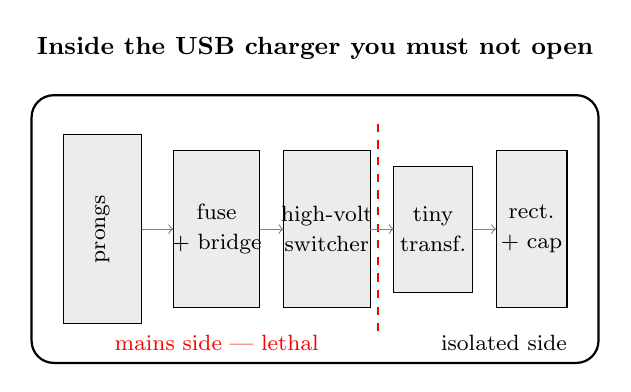
\begin{tikzpicture}[font=\small]
\draw[thick, rounded corners=8pt] (0,0) rectangle (7.2,3.4);
\node[align=center] at (3.6,4.0) {\textbf{Inside the USB charger you must not open}};
\draw[fill=gray!15] (0.4,0.5) rectangle (1.4,2.9); \node[rotate=90] at (0.9,1.7) {\footnotesize prongs};
\draw[fill=gray!15] (1.8,0.7) rectangle (2.9,2.7); \node[align=center] at (2.35,1.7) {\footnotesize fuse\\ \footnotesize + bridge};
\draw[fill=gray!15] (3.2,0.7) rectangle (4.3,2.7); \node[align=center] at (3.75,1.7) {\footnotesize high-volt\\ \footnotesize switcher};
\draw[fill=gray!15] (4.6,0.9) rectangle (5.6,2.5); \node[align=center] at (5.1,1.7) {\footnotesize tiny\\ \footnotesize transf.};
\draw[fill=gray!15] (5.9,0.7) rectangle (6.8,2.7); \node[align=center] at (6.35,1.7) {\footnotesize rect.\\ \footnotesize + cap};
\draw[dashed, thick, red] (4.4,0.4) -- (4.4,3.1);
\node[red, font=\footnotesize, align=center] at (2.35,0.25) {mains side --- lethal};
\node[font=\footnotesize, align=center] at (6.0,0.25) {isolated side};
\draw[->, gray] (1.4,1.7) -- (1.8,1.7); \draw[->, gray] (2.9,1.7) -- (3.2,1.7);
\draw[->, gray] (4.3,1.7) -- (4.6,1.7); \draw[->, gray] (5.6,1.7) -- (5.9,1.7);
\end{tikzpicture}

\caption{What is actually inside a \qty{5}{\volt} USB charger. Notice the
dashed line: everything left of it touches mains; the isolation boundary
is engineered, tested, and certified. Look — never open.}
\label{fig:wall}
\end{figure}

\begin{rulebox}[Mains: the hard boundary]
\begin{itemize}
\item \qty{230}{\volt} AC kills. It is not a bigger 9 V battery — a
mains shock across the chest can stop a heart, and a mains fault starts
fires, not sparks.
\item Never open, probe, repair, or re-use the inside of a wall
adapter, charger, or mains-powered brick — even unplugged, its
capacitors hold lethal charge for minutes.
\item Buy, don't build: USB supplies and lab bench supplies are
cheap, certified, and isolated. There is no beginner project whose
power stage should touch mains.
\item Cheap no-name chargers fail the isolation test too — buy known
brands from real shops.
\end{itemize}
\end{rulebox}

\begin{rulebox}[Battery energy: USB packs and LiPo]
USB power banks are the friendly face of lithium cells — that is why
they are allowed. The cells inside store real energy: shorted, a LiPo
sustains tens of amps and vents fire. Never pierce, crush, solder
directly on, or charge unattended loose lithium cells; use the
protected, cased packs as they come. A swollen pack is retired, not
``used up''.
\end{rulebox}

\section{Common mistakes}
\label{sec:mistakes07}

\begin{itemize}
\item \textbf{Applying the golden rules at the rails.} If the required
output exceeds the supply, the rules are already dead — check headroom
first (Section~\ref{sec:we-clip}).
\item \textbf{Forgetting decoupling capacitors.} An op-amp starved at
its supply pins oscillates mysteriously; \qty{100}{\nano\farad} across
the pins is cheap insurance, always.
\item \textbf{Using an op-amp as a comparator without hysteresis.} A
noisy input near the threshold chatters the output between rails; add
positive feedback or buy a real comparator.
\item \textbf{Expecting gain at any frequency.} GBW means a
$\times100$ amplifier is not one at \qty{100}{\kilo\hertz} — check the
bandwidth budget before the resistor ratio.
\item \textbf{Assuming the input range too.} Some parts read inputs
near the negative rail only; ``single-supply'' does not mean
``accepts any input''.
\end{itemize}

\section{Exercises}
\label{sec:exercises07}

\begin{exercise}[easy]
A buffer follows a sensor output of \qty{3.1}{\volt}. What is the
buffer's output voltage, and why would you bother if the number doesn't
change?
\end{exercise}

\begin{exercise}[easy]
An inverting amplifier has $R_{\mathrm{in}} = \qty{2}{\kilo\ohm}$,
$R_f = \qty{20}{\kilo\ohm}$. What is the gain, and what input gives
$+\qty{5}{\volt}$ out?
\end{exercise}

\begin{exercise}[easy]
A non-inverting amplifier needs gain $11$. If $R_2 = \qty{1}{\kilo\ohm}$,
choose $R_1$.
\end{exercise}

\begin{exercise}[easy]
Your op-amp is on $\pm\qty{9}{\volt}$ rails and saturates about
\qty{1.5}{\volt} inside them. You want a $\pm\qty{6}{\volt}$ sine out of
gain $20$. What is the largest input amplitude you can amplify cleanly?
\end{exercise}

\begin{exercise}[medium]
A comparator circuit has $R_1 = \qty{10}{\kilo\ohm}$ to ground and
$R_2 = \qty{30}{\kilo\ohm}$ to the output, which saturates at
$\pm\qty{10}{\volt}$. Find both switching thresholds $V_{T+}$ and
$V_{T-}$.
\end{exercise}

\begin{exercise}[medium]
Using $T = 2RC\ln\frac{1+k}{1-k}$: a relaxation oscillator runs at
\qty{250}{\hertz} with $k = 0.5$ and $C = \qty{100}{\nano\farad}$.
What is $R$?
\end{exercise}

\begin{exercise}[medium]
A project draws \qty{80}{\milli\ampere} at \qty{5}{\volt} and you can
feed the regulator \qty{9}{\volt}. Compare an LDO (dropout
\qty{0.4}{\volt}) against a buck module: which do you pick, and what
power does the loser waste? When would the answer flip?
\end{exercise}

\begin{exercise}[medium]
You need $\times50$ gain at \qty{20}{\kilo\hertz} from a
\qty{1}{\mega\hertz} GBW op-amp. Can you do it in one stage? What
open-loop gain does the chip actually offer there, and what does that
do to accuracy?
\end{exercise}

\begin{exercise}[hard]
(Implement) Extend \texttt{comparator\_osc.cir}: make $k \neq 0.5$ by
setting $R_1 = \qty{10}{\kilo\ohm}$, $R_2 = \qty{20}{\kilo\ohm}$
($k = \frac{1}{3}$). Derive the new predicted period, re-simulate, and
report measured vs predicted in a table. \textbf{Hint:}
$\ln\frac{1+k}{1-k} = \ln 2$ now.
\end{exercise}

\begin{exercise}[hard]
A \qty{12}{\volt}-to-\qty{5}{\volt} linear regulator supplies a
\qty{300}{\milli\ampere} load. Compute the dissipated power, and explain
why engineers choose a buck converter here — then explain when they
would \emph{not} (think noise, cost, battery standby).
\end{exercise}

\section{Summary}
\label{sec:summary07}

\begin{center}
\small
\begin{tabular}{@{}p{0.30\linewidth}p{0.62\linewidth}@{}}
\toprule
\textbf{Idea} & \textbf{One-line version} \\ \midrule
Golden rules & With negative feedback: inputs draw no current, and $v_+ = v_-$ — until the rails say otherwise. \\
Buffer & Copies a voltage without loading the source. \\
Inverting amp & Gain $-R_f/R_{\mathrm{in}}$; $v_-$ is a virtual ground. \\
Non-inverting amp & Gain $1 + R_1/R_2 \ge 1$; input sees no load. \\
Comparator & No taming feedback: output rails declare which input is bigger. \\
Hysteresis & Positive feedback gives two thresholds; noise can't dither the output. \\
Clipping & Demanded output beyond swing limit = flat-topped waveform. \\
Linear regulator & Burns the voltage difference as heat: simple, quiet, inefficient. \\
Switching regulator & Chops through an inductor: efficient, noisy. \\
USB supply & Pre-regulated, current-limited, safe — the book's bench supply. \\
Mains & \qty{230}{\volt} stays inside certified boxes. Buy, never build. \\
Decoupling & \qty{100}{\nano\farad} at every chip's supply pins, always. \\
\bottomrule
\end{tabular}
\end{center}

\section*{Notes}
\begin{enumerate}
\item \emph{All About Circuits}, vol.\ III, ch.\ 8 — the op-amp chapters
the buffer/inverting/comparator analyses follow~\cite{aacvol3}.
\item MIT \emph{6.002} lectures 8--12 (op-amp abstraction, negative
feedback) and 20+ (power) — the golden-rules framing and the honest
limits list~\cite{ocw6002}.
\item Horowitz \& Hill, \emph{The Art of Electronics} — the cited next
step for comparator subtleties, regulators, and real-world
op-amp pathologies~\cite{aoe}.
\end{enumerate}

\section*{Hints and answers}
\begin{description}
\item[Buffer (easy)] \qty{3.1}{\volt}. The point is the \emph{current}:
the buffer supplies load current from its rails while drawing $\sim 0$
from the sensor.
\item[Inverting gain (easy)] Gain $-10$; input $-\qty{0.5}{\volt}$.
\item[Non-inverting (easy)] $R_1 = \qty{10}{\kilo\ohm}$ ($1+10=11$).
\item[Headroom (easy)] Swing limit $\approx \pm 7.5$ V $>$ the
\qty{6}{\volt} needed; max clean input $= 6/20 = \qty{0.3}{\volt}$.
\item[Weak sensor (inline, \S\ref{sec:three})] Without buffer
$\approx \qty{0.227}{\volt}$; with buffer $\approx \qty{2.5}{\volt}$
--- the sim of \S\ref{sec:we-buffer} measures both.
\item[Mic gain (inline, \S\ref{sec:we-clip})] $R_f =
\qty{30}{\kilo\ohm}$, $R_{\mathrm{in}} = \qty{1}{\kilo\ohm}$;
$\pm 1.5$ V out is far inside the swing limit.
\item[Osc period (inline, \S\ref{sec:we-osc})] $RC = 1/(2\ln 3)\,
\mathrm{ms} \approx \qty{0.455}{\milli\second}$; e.g.\
$R = \qty{4.55}{\kilo\ohm}$, $C = \qty{100}{\nano\farad}$.
\item[Thresholds (medium)] $V_T = \frac{10}{40}\times 10 =
\pm\qty{2.5}{\volt}$: flips high at $+2.5$, low at $-2.5$.
\item[Oscillator $R$ (medium)] $R = \frac{1}{2fC\ln 3} \approx
\qty{18.2}{\kilo\ohm}$.
\item[LDO vs buck (medium)] LDO wastes $(9-5)\times 0.08 =
\qty{0.32}{\watt}$ with $4$ V of headroom $\gg$ \qty{0.4}{\volt}
dropout --- pick the LDO. Buck wins when current is amps, or battery
life beats noise.
\item[GBW (medium)] Open-loop gain at \qty{20}{\kilo\hertz} $\sim
10^{6}/2\times10^{4} = 50$ --- barely the wanted closed loop; split into
two $\times 7$ stages or choose a faster part.
\item[$k=1/3$ oscillator (hard)] $T = 2RC\ln 2 \approx
\qty{1.39}{\milli\second}$ predicted ($\approx\qty{721}{\hertz}$);
simulate and tabulate --- expect within $1\%$.
\item[Linear vs buck, \qty{300}{\milli\ampere} (hard)] $(12-5)\times
0.3 = \qty{2.1}{\watt}$ of heat --- buck territory. Skip it when noise
is critical, cost rules, or load is milliamps.
\end{description}
